\documentclass[12pt,a4paper]{article}
% Estilo compartido para informes. Compilar con LuaLaTeX desde tp1/.
\usepackage[spanish,es-nodecimaldot]{babel}
\usepackage{fontspec}
\setmainfont{Montserrat-Medium.ttf}[
  Path=../assets/fonts/,
  BoldFont=Montserrat-Bold.ttf,
  ItalicFont=Montserrat-MediumItalic.ttf]
\usepackage[a4paper,margin=2.5cm,headheight=16pt]{geometry}
\usepackage{xcolor,graphicx,booktabs,tabularx}
\usepackage{float}
\usepackage{titlesec,fancyhdr,enumitem,caption}
\usepackage{ragged2e}
\usepackage{hyperref}
\definecolor{verde}{HTML}{1D4036}
\definecolor{bronce}{HTML}{D38129}
\definecolor{rosa}{HTML}{D88E77}
\definecolor{calido}{HTML}{EFE4D8}
\definecolor{grafito}{HTML}{1D1D1D}
\hypersetup{colorlinks=true,linkcolor=verde,urlcolor=verde,
  pdftitle={TP1 - Instalación de máquinas virtuales},pdfsubject={Cyberseguridad}}
\AtBeginDocument{\color{grafito}\RaggedRight\fontsize{12}{14.4}\selectfont}
\setlength{\parindent}{0pt}
\setlength{\parskip}{7pt}
\setlist[itemize]{leftmargin=*,itemsep=7pt,topsep=4pt}
\setlist[enumerate]{leftmargin=*,itemsep=6pt}
\titleformat{\section}{\color{verde}\bfseries\fontsize{18}{21.6}\selectfont}{\thesection}{0.65em}{}
\titleformat{\subsection}{\color{verde}\bfseries\large}{\thesubsection}{0.65em}{}
\titleformat{\subsubsection}{\color{verde}\bfseries}{\thesubsubsection}{0.65em}{}
\titlespacing*{\section}{0pt}{16pt}{8pt}
\titlespacing*{\subsection}{0pt}{12pt}{5pt}
\titlespacing*{\subsubsection}{0pt}{10pt}{4pt}
\setcounter{tocdepth}{2}
\pagestyle{fancy}
\fancyhf{}
\fancyhead[L]{\small\color{verde}FCEFyN | UNC}
\fancyhead[R]{\small\color{verde}\materia\ · TP \numeroTP}
\fancyfoot[L]{\scriptsize Informe de laboratorio}
\fancyfoot[R]{\small\thepage}
\renewcommand{\headrulewidth}{0.4pt}
\captionsetup{font=small,labelfont=bf,justification=raggedright,singlelinecheck=false,hypcap=false}
\newcommand{\pendiente}[1]{\par{\small\color{verde}\textbf{Por completar.} #1\par}}
% Si falta una captura se muestra un espacio reservado; no impide compilar.
\newcommand{\captura}[2]{%
  \par\smallskip\begingroup\centering
  \IfFileExists{figuras/#1}{%
    \includegraphics[width=\linewidth,height=5cm,keepaspectratio]{figuras/#1}%
  }{%
    \setlength{\fboxsep}{10pt}%
    \fcolorbox{bronce}{calido}{\parbox[c][1.25cm][c]{\dimexpr\linewidth-2\fboxsep-2\fboxrule\relax}{%
      \centering\small Captura pendiente\par\texttt{\detokenize{#1}}}}%
  }%
  \captionof{figure}{#2}\par\endgroup\smallskip
}

\usepackage{xurl}

\newcommand{\materia}{Cyberseguridad}
\newcommand{\numeroTP}{11}
\newcommand{\tituloTP}{Seguridad en sistemas embebidos}
\newcommand{\estudiante}{Brigido Tomas Andres}
\newcommand{\legajo}{38481096}
\newcommand{\carrera}{ICOMP}
\newcommand{\docente}{Javier A. Jorge}


% Metadatos específicos del TP11 y capturas en img/.
\hypersetup{pdftitle={TP11 - Seguridad en sistemas embebidos},
    linkcolor=black,urlcolor=black,citecolor=black}
\renewcommand{\captura}[2]{%
  \begin{figure}[H]
    \centering
    \IfFileExists{img/#1}{%
      \includegraphics[width=0.85\linewidth,height=5cm,keepaspectratio]{img/#1}%
    }{%
      \setlength{\fboxsep}{10pt}%
      \fcolorbox{bronce}{calido}{\parbox[c][1.1cm][c]{0.85\linewidth}{%
        \centering\small Captura pendiente\par\texttt{\detokenize{#1}}}}%
    }%
    \caption{#2}
  \end{figure}
}

\usepackage{caption}
\captionsetup{justification=centering}
\begin{document}
\hypersetup{pageanchor=false}
\begin{titlepage}
  
\includegraphics[width=8cm]{../assets/logo-fcefyn-2026.png}
  \vspace{1cm}

  {\color{verde}\small UNIVERSIDAD NACIONAL DE CÓRDOBA\par}
  \vspace{2.1cm}
  {\color{bronce}\bfseries\large TRABAJO PRÁCTICO \numeroTP\par}
  \vspace{0.45cm}
  {\color{verde}\bfseries\fontsize{32}{38.4}\selectfont Seguridad en\\sistemas\\embebidos\par}
  \vspace{0.3cm}
{\small Incidentes y aplicaciones de criptografía\par}
\vspace{0.35cm}
  {\large \materia\par}
  \vspace{0.8cm}
  {\color{bronce}\rule{2.7cm}{2pt}\par}
  \vfill
  \renewcommand{\arraystretch}{1.45}
  \begin{tabular}{@{}p{3.2cm}p{10cm}@{}}
    Estudiante & \estudiante \\
    Legajo & \legajo \\
    Carrera & \carrera \\
    Docente & \docente \\
  \end{tabular}
  \vfill
  {\small Córdoba, Argentina\par}
\end{titlepage}
\hypersetup{pageanchor=true}

\tableofcontents
\vspace{1cm}
\newpage

\section{Problemas de seguridad frecuentes}
\textbf{1- Leer el sitio de INCIBE y revisar los problemas de seguridad más frecuentes.}

Entre los problemas de seguridad revisados se destacan los siguientes:

\begin{itemize}
    \item \textbf{Certificados autofirmados:} algunos servicios utilizan certificados sin el respaldo de una entidad de confianza. Si no se verifica su autenticidad por otro medio, puede resultar difícil confirmar la identidad del dispositivo.

    \item \textbf{Contraseñas embebidas y puertas traseras:} el fabricante puede incorporar contraseñas que no se pueden modificar y que se comparten entre dispositivos. Las puertas traseras permiten acceder mediante mecanismos alternativos que pueden eludir los controles configurados por el usuario.

    \item \textbf{Criptografía débil o inexistente:} la ausencia de cifrado o el uso de mecanismos débiles puede dejar expuesta la información almacenada o transmitida.

    \item \textbf{Vulnerabilidades en los servicios del dispositivo:} las interfaces HMI, de gestión y web pueden presentar fallos como XSS o inyección SQL. En estos casos, el dispositivo embebido actúa como servidor y recibe las solicitudes de los clientes.

    \item \textbf{Denegación de servicio (DoS y DDoS):} las solicitudes reiteradas pueden agotar los recursos del dispositivo o saturar sus comunicaciones, afectando su disponibilidad, especialmente si carece de controles adecuados.
\end{itemize}

También se identificaron otros problemas:
\begin{itemize}
    \item Fallos en componentes de código libre.
    \item Autenticación débil o inexistente.
    \item Problemas de seguridad en las comunicaciones de entrada y salida.
    \item Explotación de la lógica en escalera.
\end{itemize}

\section{Incidentes en sistemas embebidos}
\textbf{2- Buscar al menos tres casos de incidentes de seguridad en un sistema embebido e indicar cómo se pudo haber evitado.}

\subsection{Caso 1}
\textbf{Stuxnet (2010):} Un gusano informático avanzado diseñado para atacar los sistemas de control industrial (ICS) y autómatas programables (PLC) de las centrifugadoras nucleares en Irán. El malware alteraba la velocidad de giro de los motores de forma imperceptible para los operadores hasta destruir el hardware.

\subsection{Caso 2}
\textbf{Hackeo de sistemas de automóviles conectados (Jeep Cherokee, 2015):} Un grupo de investigadores demostró que se podía tomar el control de un vehículo en marcha a través de su sistema de infoentretenimiento conectado a internet (Uconnect). Mediante esta brecha, lograron manipular la transmisión, los frenos y el volante.

\subsection{Caso 3}
\textbf{Mirai (y su propagación en dispositivos IoT):} Es un malware que infecta sistemas embebidos con Linux (como cámaras de seguridad IP y routers) utilizando credenciales predeterminadas de fábrica. Una vez dentro, convierte estos dispositivos en un ejército de bots (botnet) para lanzar ataques masivos de denegación de servicio (DDoS) que tiran sitios web globales. El código fuente de Mirai puede consultarse en el repositorio publicado por jgamblin~\cite{mirai}.

\section{Práctica de criptografía}
\begin{figure}[H]
    \centering
    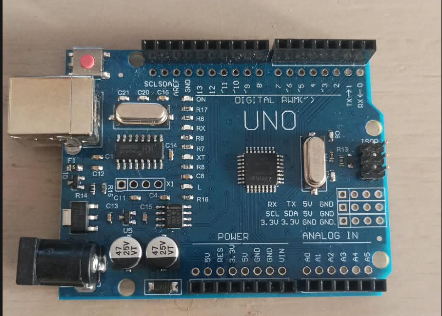
\includegraphics[width=0.9\textwidth]{img/placaArduino.png}
    \caption{Placa compatible con Arduino Uno, versión SMD, utilizada para la práctica de criptografía.}
    \label{fig:una-imagen}
\end{figure}

\newpage
\textbf{3- Realizar los ejemplos de las filminas de Seguridad en sistemas embebidos: hash, encripción simétrica y firma digital.}

\subsection{Hash}
\begin{figure}[H]
    \centering
    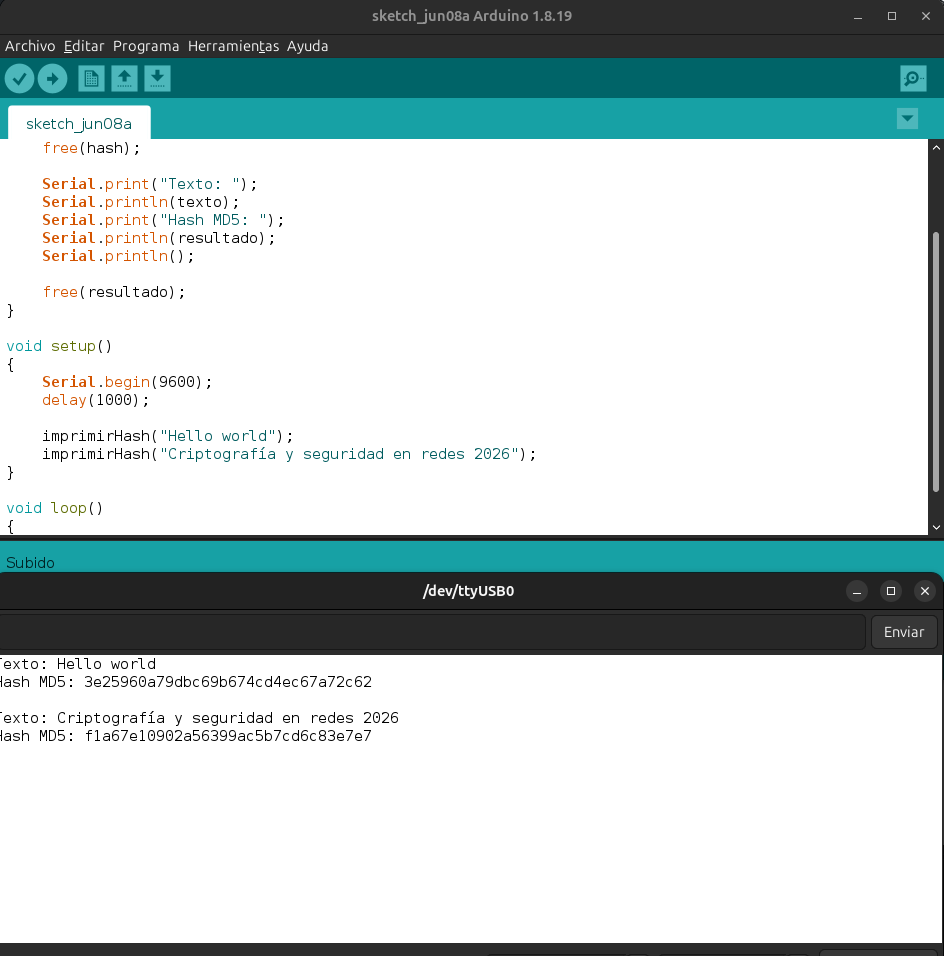
\includegraphics[width=0.9\textwidth]{img/hash.png}
    \caption{Proceso de generación de hash.}
    \label{fig:una-imagen}
\end{figure}

\newpage
\par\textbf{Código utilizado para generar el hash MD5.}
\begingroup
\small
\begin{verbatim}
#include <MD5.h>

void imprimirHash(const char* texto)
{
    unsigned char* hash = MD5::make_hash(texto);
    char* resultado = MD5::make_digest(hash, 16);
    free(hash);

    Serial.print("Texto: ");
    Serial.println(texto);
    Serial.print("Hash MD5: ");
    Serial.println(resultado);
    Serial.println();

    free(resultado);
}

void setup()
{
    Serial.begin(9600);
    delay(1000);

    imprimirHash("Hello world");
    imprimirHash("Criptografía y seguridad en redes 2026");
}

void loop()
{
    // No repetir las impresiones.
}
\end{verbatim}
\endgroup

\subsection{Encripción simétrica}
\begin{figure}[H]
    \centering
    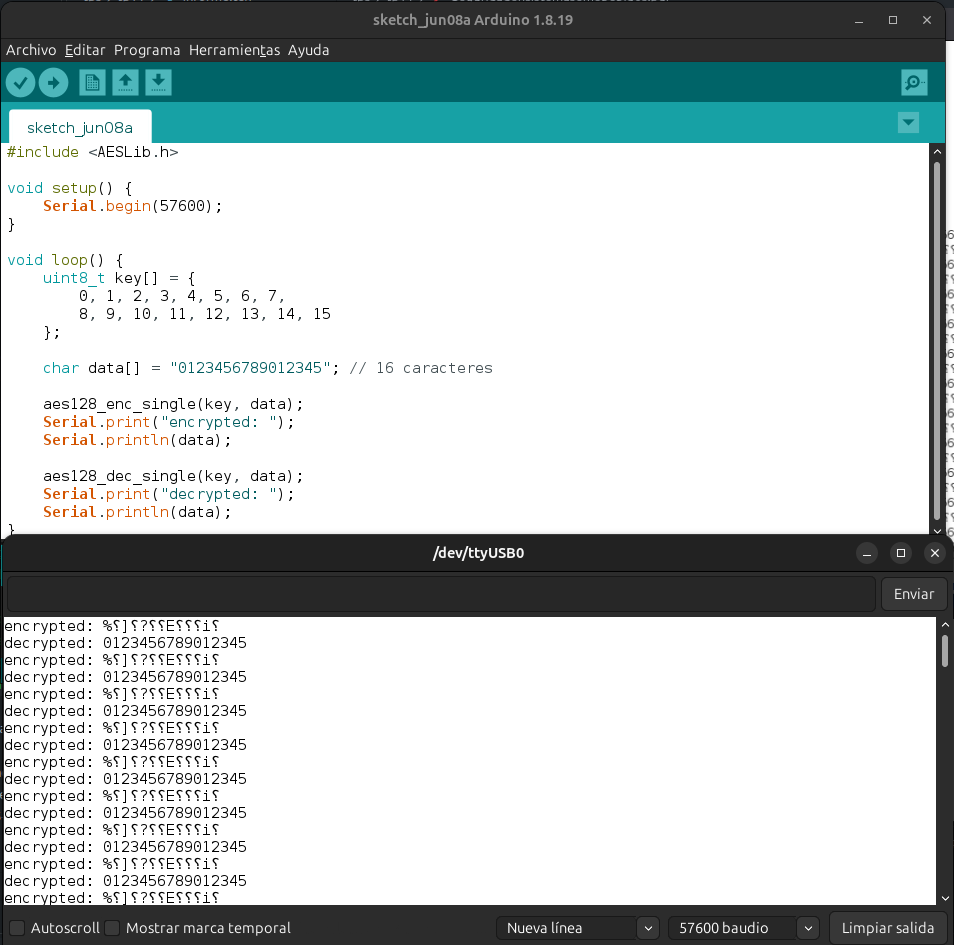
\includegraphics[width=0.9\textwidth]{img/encriptSimetrica.png}
    \caption{Proceso de encriptación simétrica.}
    \label{fig:una-imagen}
\end{figure}

\newpage
\par\textbf{Código utilizado para el cifrado simétrico AES.}
Se utiliza la biblioteca AESLib de DavyLandman~\cite{aeslib}.
\begingroup
\small
\begin{verbatim}
#include <AESLib.h>

void setup() {
    Serial.begin(57600);
}

void loop() {
    uint8_t key[] = {
        0, 1, 2, 3, 4, 5, 6, 7,
        8, 9, 10, 11, 12, 13, 14, 15
    };

    char data[] = "0123456789012345"; // 16 caracteres

    aes128_enc_single(key, data);
    Serial.print("encrypted: ");
    Serial.println(data);

    aes128_dec_single(key, data);
    Serial.print("decrypted: ");
    Serial.println(data);
}
\end{verbatim}
\endgroup

\subsection{Firma digital}
\begin{figure}[H]
    \centering
    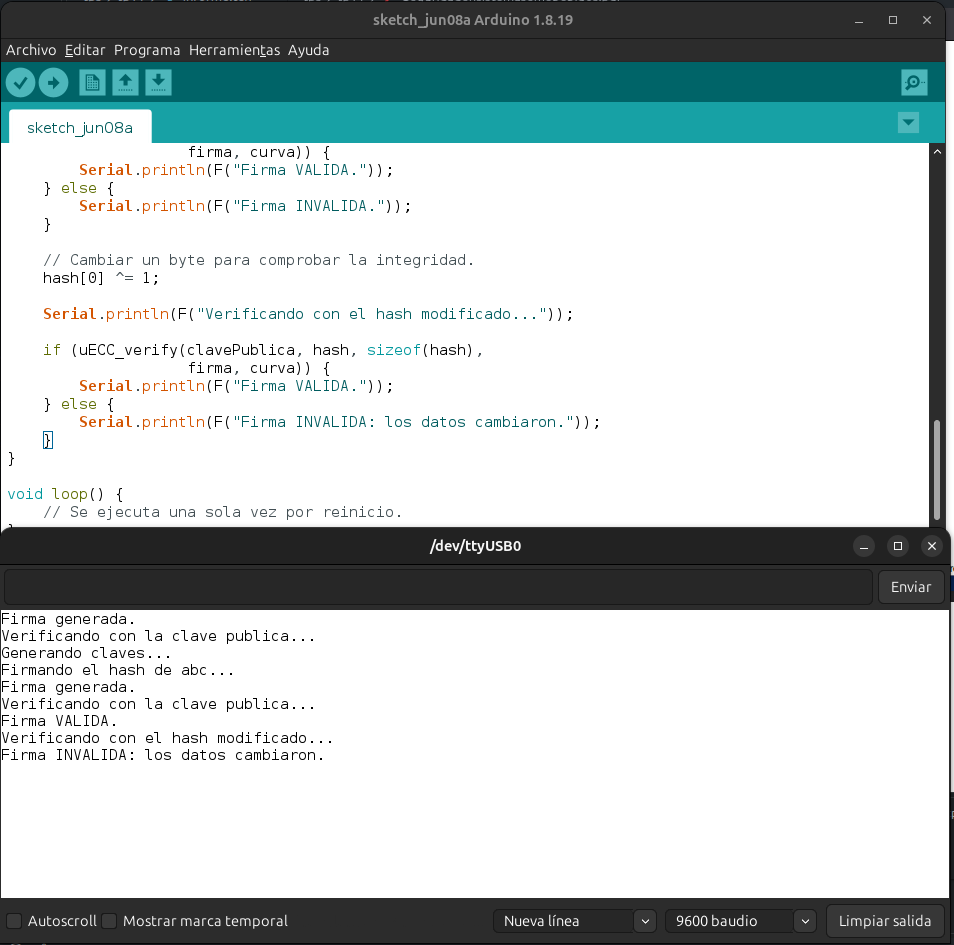
\includegraphics[width=0.9\textwidth]{img/certificado.png}
    \caption{Proceso de firma digital.}
    \label{fig:una-imagen}
\end{figure}

\newpage
\par\textbf{Código utilizado para la firma digital.}
Se utiliza la biblioteca micro-ecc de kmackay~\cite{micro-ecc}. El ejemplo firma el hash SHA-256 precalculado de \texttt{abc}, verifica la firma y repite la verificación tras modificar el hash. La aleatoriedad es predecible y se utiliza únicamente para esta demostración de laboratorio, no para proteger información real.
\begingroup
\small
\begin{verbatim}
#include <uECC.h>

// Solo para esta demostracion.
// Este generador NO es seguro para claves reales.
int generarAleatorios(uint8_t* destino, unsigned cantidad) {
    for (unsigned i = 0; i < cantidad; i++) {
        destino[i] = (uint8_t)random(256);
    }
    return 1;
}

void setup() {
    Serial.begin(9600);
    delay(1000);

    randomSeed(12345); // Prueba reproducible
    uECC_set_rng(generarAleatorios);

    // Misma curva que utiliza la filmina.
    const struct uECC_Curve_t* curva = uECC_secp160r1();

    uint8_t clavePrivada[21];
    uint8_t clavePublica[40];
    uint8_t firma[40];

    // SHA-256 del texto "abc", precalculado.
    uint8_t hash[32] = {
        0xba, 0x78, 0x16, 0xbf, 0x8f, 0x01, 0xcf, 0xea,
        0x41, 0x41, 0x40, 0xde, 0x5d, 0xae, 0x22, 0x23,
        0xb0, 0x03, 0x61, 0xa3, 0x96, 0x17, 0x7a, 0x9c,
        0xb4, 0x10, 0xff, 0x61, 0xf2, 0x00, 0x15, 0xad
    };

    Serial.println(F("Generando claves..."));

    if (!uECC_make_key(clavePublica, clavePrivada, curva)) {
        Serial.println(F("Error al generar las claves."));
        return;
    }

    Serial.println(F("Firmando el hash de abc..."));

    if (!uECC_sign(clavePrivada, hash, sizeof(hash),
                   firma, curva)) {
        Serial.println(F("Error al generar la firma."));
        return;
    }

    Serial.println(F("Firma generada."));
    Serial.println(F("Verificando con la clave publica..."));

    if (uECC_verify(clavePublica, hash, sizeof(hash),
                    firma, curva)) {
        Serial.println(F("Firma VALIDA."));
    } else {
        Serial.println(F("Firma INVALIDA."));
    }

    // Cambiar un byte para comprobar la integridad.
    hash[0] ^= 1;

    Serial.println(F("Verificando con el hash modificado..."));

    if (uECC_verify(clavePublica, hash, sizeof(hash),
                    firma, curva)) {
        Serial.println(F("Firma VALIDA."));
    } else {
        Serial.println(F("Firma INVALIDA: los datos cambiaron."));
    }
}

void loop() {
    // Se ejecuta una sola vez por reinicio.
}
\end{verbatim}
\endgroup

El programa genera un par de claves y firma el hash de prueba con la clave privada. Luego verifica la firma con la clave pública. Al modificar un byte del hash, la verificación falla, mostrando que la firma permite detectar cambios en los datos. Todo se ejecuta una sola vez en \texttt{setup()}.


\newpage
\renewcommand{\refname}{Referencias}
\begin{thebibliography}{9}
\addcontentsline{toc}{section}{Referencias}
\bibitem{mirai} jgamblin. \textit{Mirai-Source-Code}. GitHub.
\url{https://github.com/jgamblin/Mirai-Source-Code}.
\bibitem{incibe-embebidos} INCIBE. \textit{Introducción a los sistemas embebidos}.
\url{https://www.incibe.es/incibe-cert/blog/introduccion-los-sistemas-embebidos}.
\bibitem{seguridad-embebidos} \textit{Seguridad en sistemas embebidos}. ResearchGate.
\url{https://www.researchgate.net/publication/327163345_Seguridad_en_sistemas_embebidos}.
\bibitem{arduino-md5} tzikis. \textit{ArduinoMD5}. GitHub.
\url{https://github.com/tzikis/ArduinoMD5}.
\bibitem{aeslib} DavyLandman. \textit{AESLib}. GitHub.
\url{https://github.com/DavyLandman/AESLib}.
\bibitem{micro-ecc} kmackay. \textit{micro-ecc}. GitHub.
\url{https://github.com/kmackay/micro-ecc}.
\end{thebibliography}

\end{document}
